\documentclass{article}
\usepackage{latexsym}
\usepackage[utf8]{inputenx}
\usepackage[spanish]{babel}
\usepackage{graphicx}
\usepackage{anysize}
\usepackage{amsmath}
\usepackage{amssymb}
\usepackage{float}
\setlength{\skip\footins}{5cm}
\usepackage{lscape}
\usepackage{verbatim}
\usepackage{moreverb}
\usepackage{url}
\usepackage{enumitem}
\usepackage{multicol}
\let\verbatiminput=\verbatimtabinput
\usepackage[nottoc,numbib]{tocbibind}
\setcounter{tocdepth}{4}
\setcounter{secnumdepth}{4}

\marginsize{2cm}{2cm}{.5cm}{3cm} 

\begin{document}

\begin{titlepage}

\newcommand{\HRule}{\rule{\linewidth}{0.5mm}} % Defines a new command for the horizontal lines, change thickness here

\center % Center everything on the page
 
%----------------------------------------------------------------------------------------
%	HEADING SECTIONS
%----------------------------------------------------------------------------------------

\textsc{\LARGE Universidad De Buenos Aires}\\[1.5cm] % Name of your university/college
\textsc{\Large Facultad De Ingeniería}\\[0.5cm] % Major heading such as course name
\textsc{\large 75.52 Taller de Programaci\'on II}\\[0.5cm] % Minor heading such as course title

%----------------------------------------------------------------------------------------
%	TITLE SECTION
%----------------------------------------------------------------------------------------

\HRule \\[0.4cm]
{ \huge \bfseries Recursos}\\ Capa de Negocios\\[0.4cm] % Title of your document
\HRule \\[1.5cm]
 
%----------------------------------------------------------------------------------------
%	AUTHOR SECTION
%----------------------------------------------------------------------------------------

% If you don't want a supervisor, uncomment the two lines below and remove the section above
\Large \emph{Integrantes:}\\

Hugo \textsc{Chavar} - 99999\\ % Your name
Dami\'an \textsc{Manoff} - 93169\\ % Your name
Yamila \textsc{Glinsek} - 99999\\ % Your name
Andr\'es \textsc{Sanabria} - 99999\\[5cm] % Your name


%----------------------------------------------------------------------------------------
%	DATE SECTION
%----------------------------------------------------------------------------------------

{\large \text \em {10 de Septiembre de 2013}}\\[3cm] % Date, change the \today to a set date if you want to be precise
 
%----------------------------------------------------------------------------------------

\vfill % Fill the rest of the page with whitespace

\end{titlepage}

\section{Introducci\'on}
Recursos da referencia a lo que podemos traducir como Archivos, Links y Encuestas.\\
Los servicios que brindamos son:
\begin{enumerate}
	\item Posibilitar la subida y descarga de archivos al sistema.
	\item Crear y Responder encuestas.
	\item Linkear paginas externas y/o internas de la web
\end{enumerate}

\section{Diagrama de Clases}
	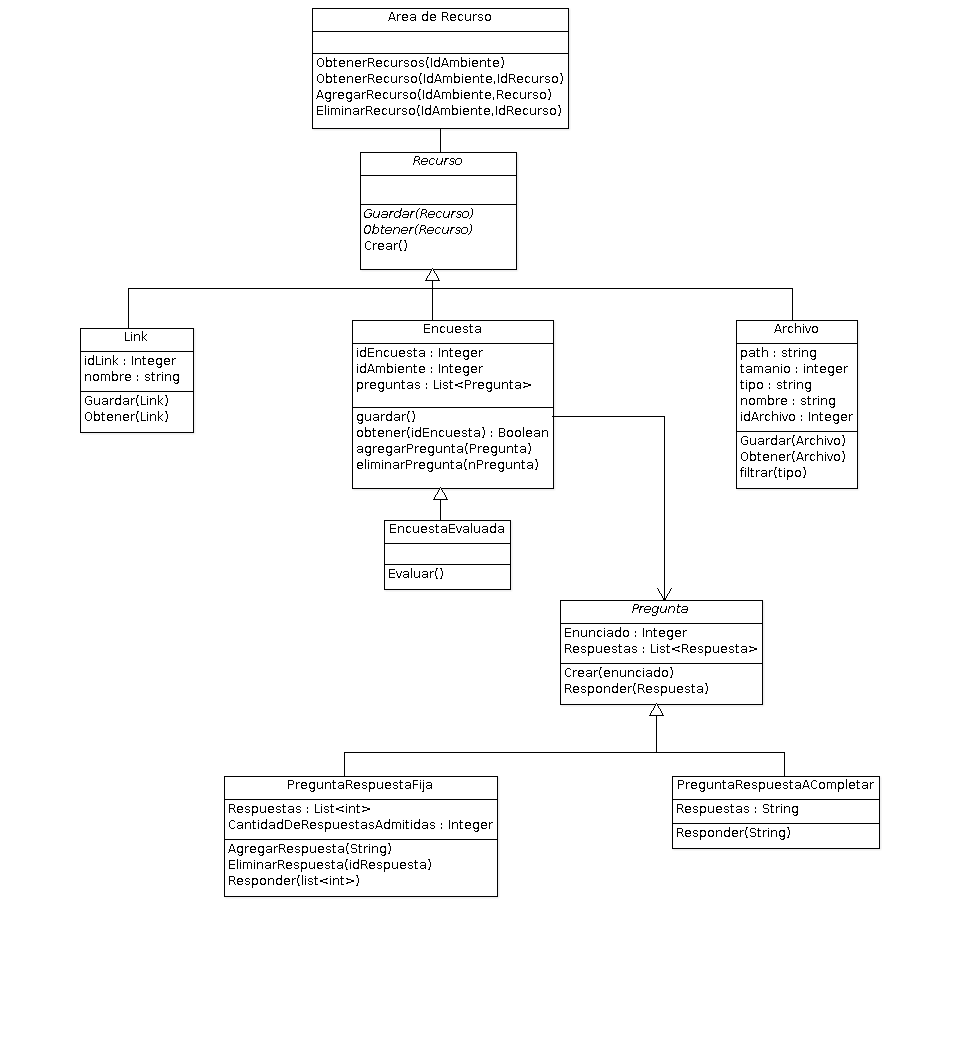
\includegraphics[scale=0.5]{Diagramadeclase2.png}
\end{document}
